\section{Problema 2}
\begin{frame}{Contenido}
        \tableofcontents[sections={3}]
\end{frame}
\subsection{Presentación del problema}
\begin{frame}{Presentación del problema}
    \begin{columns}
        \begin{column}{0.47\textwidth}
            En la siguiente figura se muestra un muro de concreto:
            \begin{figure}[h]
                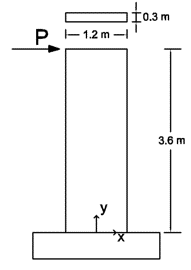
\includegraphics[width=3cm]{Imagenes/MuroEmpot.png}
                \centering
            \end{figure}
        \end{column}
        \begin{column}{0.47\textwidth}
            \justify
            El muro tiene una cimentación en la base que se considera que proporciona la condición de empotramiento. \\
            Sobre el muro se aplica una carga lateral en la parte superior. \\
            Las dimensiones del muro y su sección transversal se muestran en la figura.\\
            La resistencia a compresión del concreto es $210\frac{Kgf}{cm^{2}}$.\\
            Buscar en la literatura valores confiables de módulo de rotura del concreto, coeficiente de poisson, módulo de elasticidad y demás propiedades que necesite para los cálculos.
        \end{column}
    \end{columns}
             
\end{frame}
\subsection{Cálculo de la primera grieta}
\subsection{Cálculo de carga lateral}
\subsection{Cálculo de agrietamientos en dos puntos del muro}
\subsection{Importancia de la catenaria}
